\documentclass[a4paper, 12pt]{article}

\usepackage[utf8]{inputenc}   
\usepackage[T1]{fontenc}
\usepackage[french]{babel}

\usepackage{setspace}

\usepackage{wrapfig}
\usepackage{graphicx}
\usepackage{color}
\usepackage{eurosym}
\usepackage{multirow}
\usepackage{slashbox}
\usepackage{array}
\usepackage{colortbl}
\usepackage{lmodern}
\usepackage{amsthm}
\usepackage{amsmath}
\usepackage{amssymb}
\usepackage{mathrsfs}
\usepackage{xfrac}

\usepackage{caption}
\captionsetup{font=footnotesize}

\usepackage{subcaption}

\usepackage[colorlinks=true, linkcolor=black]{hyperref}
\usepackage{xcolor}

\usepackage[top=1.5cm, bottom=1.5cm, left=1.5cm, right=1.5cm]{geometry}

\usepackage{changepage}

\title {Étude graphique de la dérivée arithmétique}
\author{Zac Assoumani}
\date{12 février 2020}

\newcommand{\N}{\mathbb{N}}
\newcommand{\R}{\mathbb{R}}
\newcommand{\Q}{\mathbb{Q}}
\newcommand{\Pm}{\mathbb{P}}
\newcommand{\Prv}{\noindent{\it Preuve. }}
\newcommand{\cqfd}{\rule{0.2cm}{0.2cm}}
\newtheorem{prop}{Proposition}
\newtheorem{lem}{Lemme}
\newtheorem{cor}{Corollaire}
\newtheorem*{conj}{Conjecture}





\begin{document}

\maketitle

\begin{adjustwidth}{60pt}{60pt}
\begin{center}{\bf Abstract} \\
À partir de deux hypothèses sur une fonction d'entiers, on va en déduire des propositions mathématiques, avec des jolies représentations graphiques et des motifs en tous genres. \\
\end{center}
\end{adjustwidth}

\tableofcontents

\section{La dérivée arithmétique $d$}
On définit la dérivée arithmétique comme une application $d: \N \longrightarrow \N$ respectant les deux règles suivantes :
\begin{itemize}
\item
 $\forall p \in \Pm, d(p)=1$
 \item
 $\forall (a,b) \in \N^{2}, d(ab)=ad(b)+bd(a).$ \\
 \end{itemize}

\begin{lem} \label{lem1}
Pour tout n entier et k entier non-nul,
\[d(n^{k})=kn^{k-1}d(n). \]
\end{lem}
\Prv Trivial pour $k=1$.\\
Par hérédité, $d(n^{k+1}) = d(nn^{k}) = nd(n^{k})+n^{k}d(n) = kn^{k}d(n)+n^{k}d(n) = (k+1)n^{k}d(n).$  \cqfd \\


\begin{prop} \label{prop1}
Une telle fonction existe, est unique, et se définit ainsi :
\begin{itemize}
\item
$d(0)=d(1)=0$
\item
pour $n \ge 2$, si $n=\prod_{i=1}^{k} p_i^{\alpha_i}$ est la décomposition de n en facteurs premiers, alors
\begin{equation} \label{eq1}d(n)=n\sum_{i=1}^{k} \frac{\alpha_i}{p_i}. \end{equation}
\end{itemize}
\end{prop}

\Prv
\fbox{Unicité :}
\begin{itemize}
\item $d(0)=d(0^{2})=0d(0)=0$
\item $d(1)=d(1^{2})=2d(1) \Rightarrow d(1)=0$

\item
$n \ge 2$ : vrai pour $k=1$.\\
	Par hérédité si $n = \prod_{i=1}^{k+1} p_i^{\alpha_i}$ et d'après la seconde règle,

\[d(n) = {p_{k+1}}^{\alpha_{k+1}}d(\prod_{i=1}^{k} p_i^{\alpha_i}) + d({p_{k+1}}^{\alpha_{k+1}}) \prod_{i=1}^{k} p_i^{\alpha_i}.\]
Puis d'après le lemme \ref{lem1} et l'hypothèse de récurrence,
      \[d(n) = {p_{k+1}}^{\alpha_{k+1}} \prod_{i=1}^{k} p_i^{\alpha_i} \sum_{i=1}^{k} \frac{\alpha_i}{p_i} + \alpha_{k+1}{p_{k+1}}^{\alpha_{k+1}-1}  \prod_{i=1}^{k} p_i^{\alpha_i} = \]
      \[({p_{k+1}}^{\alpha_{k+1}} \prod_{i=1}^{k} p_i^{\alpha_i}) (\sum_{i=1}^{k} \frac{\alpha_i}{p_i} + \frac{\alpha_{k+1}}{p_{k+1}}) = n \sum_{i=1}^{k+1} \frac{\alpha_i}{p_i}. \]
\end{itemize}

\fbox{Existence :}\\
\underline{$d(\N) \subset \N :$} $d(n) = \sum_{i=1}^{k} \underbrace{\alpha_i \frac{n}{p_i}}_{\in \N} \in \N$.\\
\underline{$d(\Pm) = \{1\} :$} $n$ n'a qu'un seul facteur premier, lui-même, et de coefficient 1. Donc \[d(n) = n \frac{1}{n}=1.\] Puisque $\Pm$ est non-vide son image ne l'est pas non plus, d'où l'inclusion inverse.\\\\
\underline{$d(ab)=ad(b)+bd(a) :$} \begin{itemize}
\item Si $a=0$ et $b \in \N$, $d(0b)=0d(b)+bd(0)=0.$
\item Si $a=1$ et $b \in \N$, $d(1b)=1d(b)+bd(1)=d(b).$
\item Si $a=\prod_{i=1}^{k} p_i^{\alpha_i} \ge2$ et $b= \prod_{i=1}^{k} p_i^{\beta_i}\ge2$,
\[ d(ab) = d(\prod_{i=1}^{k} p_i^{\alpha_i+\beta_i}) = (\prod_{i=1}^{k} p_i^{\alpha_i+\beta_i})(\sum_{i=1}^{k} \frac{\alpha_i+\beta_i}{p_i}) = (ab\sum_{i=1}^{k} \frac{\alpha_i}{p_i}) + (ab\sum_{i=1}^{k} \frac{\beta_i}{p_i}) = ad(b)+bd(a). \] \cqfd
\end{itemize}



\begin{figure}[ht]
\begin{center}
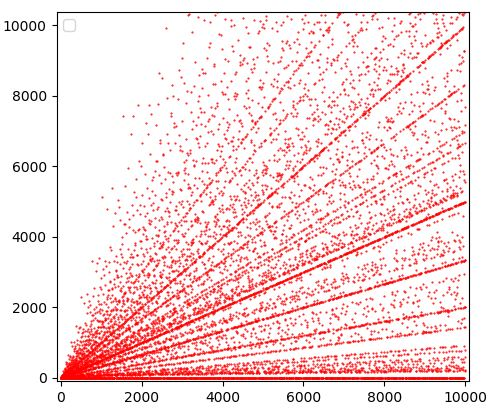
\includegraphics[scale=0.8]{graphed1.png}
\end{center}
\caption{\footnotesize{Aperçu du nuage des points $(n, d(n))$ pour $n \le 10000$.}}
\label{nuage 1}
\end{figure}


% % % % % % % % % % % % % % % % % % % % % % % % % % % % % % % %
% % % % % % % % % % % % % % % % % % % % % % % % % % % % % % % %
\newpage

\section{Représentation graphique de $d$}

La représentation graphique de $d$ (figure \ref{nuage 1}) met en avant l'abondance de points sur certaines droites, comme celles de pentes 0, 1, \sfrac{1}{2}, \sfrac{1}{3} ou \sfrac{3}{2} parmi bien d'autres. \\

% % % % % % % % % % % % % % % % % % % % % % % % % % % % % % % %

\subsection{Les "droites" $A_n$}

Pour $n \in \N^{*}$, on définit $A_n= \{(np, d(np)) \mid p \in \Pm \}$.

\begin{figure}[ht]
\begin{center}
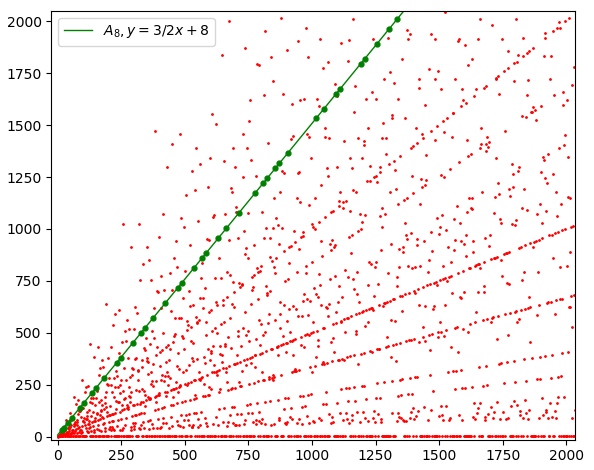
\includegraphics[scale=0.5]{graphed2.png}
\end{center}
\caption{\footnotesize{Points de $A_8$ pour $8p \le 2000$.}}
\label{nuage 2}
\end{figure}

\begin{prop} \label{prop2}
Pour tout entier $n$ non-nul, $A_n$ est inclus dans le graphe de la fonction affine d'équation \begin{equation} \label{eq2} y=\frac{d(n)}{n} x + n. \end{equation}
\end{prop}

\Prv Soit $p \in \Pm$.
\[d(np) = pd(n)+n = \frac{d(n)}{n} np + n.\]
Donc le point $(np, d(np))$ appartient au graphe de la fonction susnommée. \cqfd \\ \\

\begin{prop} \label{prop3}
Pour tout entier $n$ ayant au moins deux facteurs premiers distincts,
\begin{equation} \label{eq3} \bigcap_{\stackrel {p/n}{p \in \Pm}}^{} A_{n/p}= \{(n, d(n))\}. \end{equation}
\end{prop}

\Prv \\

\fbox{$\supset$ :}
$ p/n \Rightarrow (\frac{n}{p}p, d(\frac{n}{p}p)) = \{(n, d(n))\} \in A_{n/p}$.

\fbox{$\subset$ :}
Il existe au moins deux droites $A_{n/p}$ distinctes, leur intersection est donc un point ou l'ensemble vide. Or elle contient $\{(n, d(n))\}$. \cqfd \\

\begin{figure}[!ht]
\begin{center}
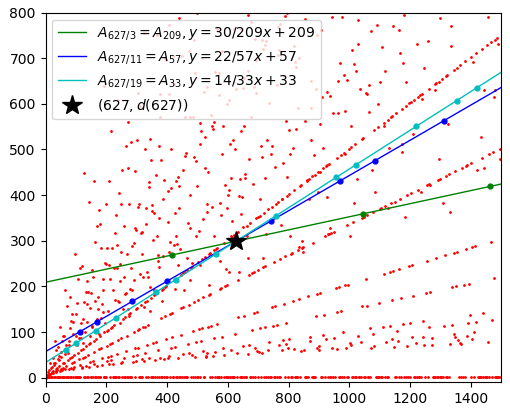
\includegraphics[scale=0.7]{graphed3.png}
\end{center}
\caption{\footnotesize{Illustration de (\ref{eq3}) pour $n=627$.}}
\label{nuage 3}
\end{figure}

% % % % % % % % % % % % % % % % % % % % % % % % % % % % % % % %

\subsection{Encadrement des valeurs}
\begin{lem}\label{lem2} Si n est produit de k facteurs premiers, alors
\[ d(n) \ge k n^{\frac{k-1}{k}}. \] \end{lem}

\Prv On peut écrire n sous la forme $n = \prod_{i=1}^{k} p_{a_i}$, donc
\[ d(n) = n \sum_{i=1}^{k} \frac{1}{p_{a_i}} = \sum_{i=1}^{k} (\prod_{j \neq i}^{} p_{a_j}). \]
La moyenne arithmétique étant supérieure à la moyenne arithmétique,
\[ d(n) \ge k (\prod_{i=1}^{k} \mbox{\small{$\prod_{j \neq i}^{} p_{a_j}$}})^k = k n^{\frac{k-1}{k}}. \] \cqfd

\begin{lem}\label{lem3} Pour tout $n \ge 2$ se décomposant en $n=\prod_{i=1}^{k} p_i^{\alpha_i}$,
\[ \sum_{i=1}^{k} \alpha_i \le \log_2(n). \] \end{lem}

\Prv Par croissance du logarithme sur $\R_{+}^{*}$,
\[ \log_2(\prod_{i=1}^{k} p_i^{\alpha_i}) \ge \log_2(\prod_{i=1}^{k} 2^{\alpha_i}) =  \sum_{i=1}^{k} \alpha_i. \] \cqfd


\begin{prop}\label{prop4} Pour $n \ge 4$ non-premier,
\begin{equation} \label{eq4}
2 \sqrt{n}\le d(n) \le \frac{n \log_2(n)}{2}. \end{equation}
\end{prop}


\Prv \\

\fbox{$2 \sqrt{n}\le d(n)$ :} $n$ est facteur de k facteurs premiers, avec $k \ge 2$ puisque $n \notin \Pm$.\\Donc d'après le lemme \ref{lem2}
\[ d(n) \ge k n^{\frac{k-1}{k}} \ge 2 \sqrt{n}.\]

\fbox{$d(n) \le \frac{n \log_2(n)}{2}$ :}
\[ d(n)=n\sum_{i=1}^{k} \frac{\alpha_i}{p_i} \le n\sum_{i=1}^{k} \frac{\alpha_i}{2} = \frac{n}{2} \sum_{i=1}^{k} \alpha_i.\]
Le résultat se déduit directement du lemme \ref{lem3}. \cqfd \\

Il y a cas d'égalité pour la borne inférieure si $n$ est le carré d'un nombre premier, et pour la borne supérieure si $n$ est de la forme $n=2^k$ avec $k$ un entier (figure \ref{nuages4}).


\begin{figure}[ht]
    \centering
    \begin{subfigure}[b]{0.3\textwidth}
        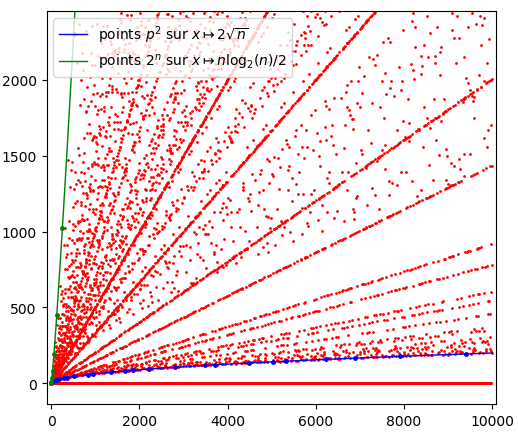
\includegraphics[width=\textwidth]{graphed4a.png}
    \end{subfigure}
    \begin{subfigure}[b]{0.3\textwidth}
        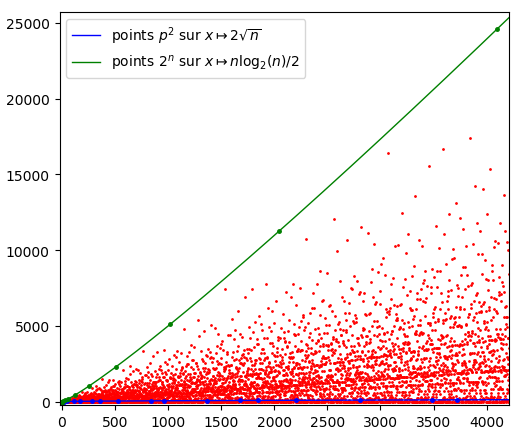
\includegraphics[width=\textwidth]{graphed4b.png}
    \end{subfigure}
    \caption{Encadrement de la fonction $d$.}
 \label{nuages4}
\end{figure}


\begin{cor}\label{cor1} $\forall n\ge2$,
\[ d^{-1}(n) \subset [\![0, \frac{n^2}{4}]\!]. \]
\end{cor}
\Prv 
\[d(a)=n \Rightarrow n \ge 2\sqrt{a} \Rightarrow \frac{n^2}{4} \ge a. \] \cqfd \\

\begin{cor} Tout $n\ge2$ possède un nombre fini d'antécédents par $d$. \end{cor}
\Prv $d^{-1}(n)$ est inclus dans un ensemble fini. \cqfd \\

\begin{cor} $d$ n'est pas surjective. \end{cor}
\Prv Montrons pour cela que 2 n'a pas d'antécédent par la fonction d. D'après le corollaire \ref{cor1},
\[d^{-1}(2) \subset [\![0, 1\!]. \]
Or \[ d([\![0, 1]\!]) = \{0\} \]
Donc \[ d^{-1}(2) \subset d^{-1}(d([\![0, 1]\!])) = d^{-1}(0). \]
Ainsi $d^{-1}(2) \subset (d^{-1}(0) \cap d^{-1}(2)) = \varnothing$. \cqfd




% % % % % % % % % % % % % % % % % % % % % % % % % % % % % % % %
% % % % % % % % % % % % % % % % % % % % % % % % % % % % % % % %



\section{La dérivée logarithmique $dl$}
\subsection{Généralités}

On définit la dérivée logarithmique \[dl : \N^{*} \longrightarrow \R, n \mapsto \frac{d(n)}{n} = \sum_{i=1}^{k} \frac{\alpha_i}{p_i}. \]

\begin{prop} \label{prop5}
$\forall (a,b) \in \N^{2},$
 \begin{equation} \label{eq5} dl(ab)=dl(a)+dl(b).
\end{equation}
\end{prop}
\Prv \[dl(ab) = \frac{d(ab)}{ab}=\frac{ad(b)+bd(a)}{ab}=\frac{d(a)}{a}+\frac{d(b)}{b}=dl(a)+dl(b).\] \cqfd



\begin{figure}[ht]
\begin{center}
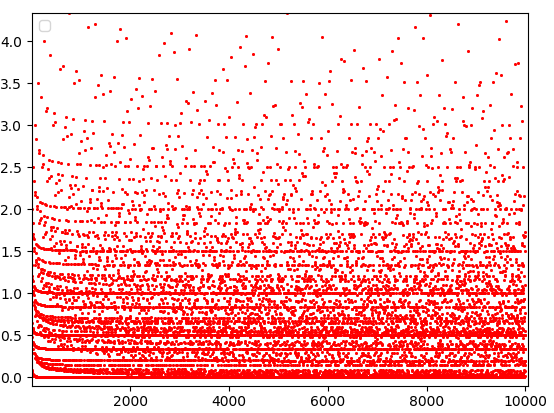
\includegraphics[scale=0.8]{graphedn1.png}
\end{center}
\caption{\footnotesize{Aperçu du nuage des points $(n, dl(n))$ pour $n \le 10000$.}}
\label{nuagen 1}
\end{figure}

% % % % % % % % % % % % % % % % % % % % % % % % % % % % % % % %

On peut remarquer la présence de courbes quasiment horizontales sur sa représentation graphique.\\
\subsection{Les "courbes" $A'_n$}
Pour $n \in \N^{*}$, on définit $A'_n= \{(np, dl(np)) \mid p \in \Pm \}.$

\begin{prop} \label{prop6}
Pour tout entier $n$ non-nul, $A'_n$ est inclus dans le graphe de la fonction d'équation \begin{equation} \label{eq6} y=dl(n) + \frac{n}{x}. \end{equation}
\end{prop}

 \Prv Soit $p \in \Pm$.
\[dl(np) = dl(n)+dl(p) = dl(n)+\frac{1}{p} = dl(n)+\frac{n}{np}. \]
Donc le point $(np, dl(np))$ appartient au graphe de la fonction susnommée. \cqfd \\ \\

Graphiquement, cela correspond bien à une courbe dont l'ordonnée tend vers $dl(n)$, qui est également la valeur de la pente associée à $A_n$.


\begin{figure}[!ht]
\begin{center}
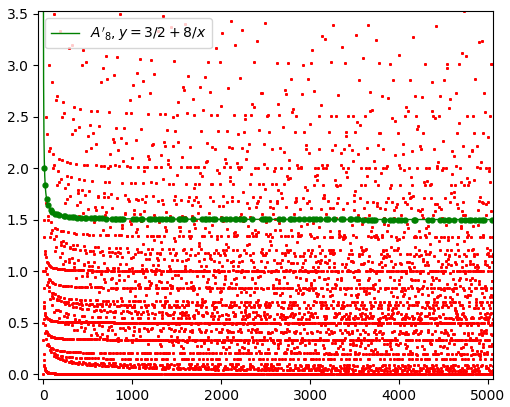
\includegraphics[scale=0.6]{graphedn2.png}
\end{center}
\caption{\footnotesize{Points de $A'_8$ pour $8p \le 10000$.}}
\label{nuagen2}
\end{figure}


% % % % % % % % % % % % % % % % % % % % % % % % % % % % % % % %

\subsection{L'ensemble $L_d$}
On définit $L_d = \{dl(n) \mid n \in \N^{*} \}$. D'après (\ref{eq2}), $L_d$ représente également l'ensemble des pentes des droites associées aux $A_n$. \\


\begin{prop} \label{prop7}
\begin{equation} \label{eq7} L_d \varsubsetneq \Q^{+}. \end{equation}
\end{prop}

\Prv \\
\fbox{$ L_d \subset \Q^{+}$ :}
$\forall n \in \N^{*}, d(n) \in \N \Rightarrow \frac{d(n)}{n} \in \Q^{+}$.\\
\fbox{$\Q^{+} \not\subset L_d$ :} Montrons par l'absurde que $\sfrac{1}{4} \notin L_d$.\\
On suppose qu'il existe des nombres premiers $p_1 \dots p_k$ et des coefficients entiers non-nuls $\alpha_1 \dots \alpha_k$ tels que $r=\sum_{i=1}^{k} \frac{\alpha_i}{p_i} = \sfrac{1}{4}$.\\
2 ne peut faire partie de ces nombres premiers, car si tel est le cas alors $r \ge \sfrac{1}{2} > \sfrac{1}{4}$. Ainsi les $p_1 \dots p_k$ sont tous impairs, donc le dénominateur de r l'est aussi et se trouve de ce fait irréductible à 4 $\Rightarrow$ contradiction.\\
r ne peut donc pas être égal à $\sfrac{1}{4}.$ \cqfd \\


\begin{prop} \label{prop8} \begin{equation}\label{eq8} \text{$L_d$ est dense dans $\R_{+}$.} \end{equation} \end{prop}

\Prv
\fbox{0 valeur d'adhérence :} Les ordonnées de $A'_1$ tendent vers 0. \\

\fbox{$a>0$ valeur d'adhérence :} Pour tout $\epsilon >0$, on peut trouver $N_0$ tel que $p_{N_0}>\frac{2}{\epsilon}$. On a l'inégalité
\[a \le \frac{\lfloor ap_{N_0} \rfloor}{p_{N_0}} < a+\frac{1}{p_{N_0}} < a + \frac{\epsilon}{2}. \]
Ainsi pour tout $n>N_0$, le $n^{ème}$ point de $A'_{p_{N_0}^{ \lfloor ap_{N_0} \rfloor}}$, est d'abscisse
\[x_n={p_{N_0}^{\lfloor ap_{N_0} \rfloor}} p_n \]
et d'ordonnée
\[y_n=dl(x_n)= \underbrace{\frac{\lfloor ap_{N_0} \rfloor}{p_{N_0}}}_{\in ]a, a+\epsilon[} + \underbrace{\frac{1}{p_n}}_{<\frac{\epsilon}{2} \text{ pour $n>N_0$}} \in ]a, a+\epsilon[ \text{ à partir d'un certain rang.}\]
En faisant tendre $\epsilon \rightarrow 0$, on peut obtenir une suite d'ordonnées (appartenant à $L_d$) tendant vers $a$. \cqfd \\ \\

% % % % % % % % % % % % % % % % % % % % % % % % % % % % % % % %

\subsection {Les "courbes" $B_{p,n}$}

Pour $n \in \N^{*}$ et $p \in \Pm$, on définit $B_{p,n}= \{(np^{k}, dl(np^{k})) \mid k \in \N \}.$

\begin{prop} \label{prop9}
Pour tout entier $n$ non-nul, $B_{p,n}$ est inclus dans le graphe de la fonction d'équation \begin{equation} \label{eq9} y=\frac{\log_p(\frac{x}{n})}{p} + dl(n). \end{equation}
\end{prop}

\Prv Soit  $n \in \N^{*}$, $p \in \Pm$ et $k \in \N$.
\[dl(np^{k}) = dl(p^k) + dl(n) = \frac{k}{p} + dl(n) = \frac{\log_p(\frac{np^{k}}{n})}{p} + dl(n).\]
Donc le point $(np^{k}, dl(np^{k}))$ appartient au graphe de la fonction susnommée. \cqfd \\

\begin{figure}[ht]
\begin{center}
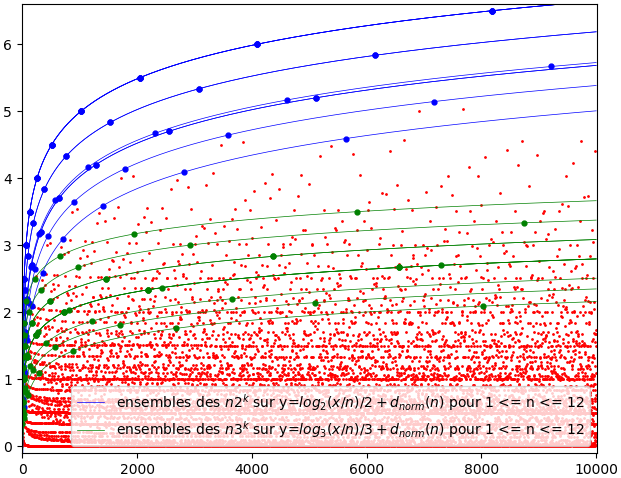
\includegraphics[scale=0.6]{graphedn3.png}
\end{center}
\caption{\footnotesize{ Points des $B_{p,n}$ pour $p=2$ et $p=3$ et pour $1 \le n \le 12$.}}
\label{nuagen 3}
\end{figure}


% % % % % % % % % % % % % % % % % % % % % % % % % % % % % % % %

\subsection{Répartition des valeurs}

On définit $M_N = \frac{1}{N} \sum_{n=1}^{N} dl(n)$ comme la moyenne des termes $\{dl(1) \dots dl(N)\}$.

\begin{prop} \label{prop10} \begin{equation} \label{eq10}
\lim_{N \to \infty} M_N = \sum_{p \in \Pm}^{} \frac{1}{p(p-1)} \approx 0.773155. \end{equation} \end{prop}

\Prv
On définit $\alpha_k : \N^{*} \longrightarrow \R$ la fonction qui a un entier $n$ non-nul associe sa valuation $p_k$-adique.
\[M_N = \frac{1}{N} \sum_{n=1}^{N} \sum_{k=1}^{\pi(N)} \frac{\alpha_k(n)}{p_k} = \frac{1}{N} \sum_{k=1}^{\pi(N)} \frac{1}{p_k} \sum_{n=1}^{N} \alpha_k(n). \]

Or \[ \sum_{n=1}^{N} \alpha_k(n) =  \sum_{i=1}^{\lfloor \frac{\log(N)}{\log(p_k)} \rfloor} i \times card(\{n \in [\![1, N]\!] \mid \alpha_k(n)=i\}) = \]
\[ \sum_{i=1}^{\lfloor \frac{\log(N)}{\log(p_k)} \rfloor} i \times card(\{n \in [\![1, N]\!] \mid {p_k}^i / n \land \lnot({p_k}^{i+1} / n)\}) = \sum_{i=1}^{\lfloor \frac{\log(N)}{\log(p_k)} \rfloor} i \left(\left\lfloor \frac{N}{{p_k}^i} \right\rfloor - \left\lfloor \frac{N}{{p_k}^{i+1}} \right\rfloor \right).\]

On peut encadrer cette expression
\[\sum_{i=1}^{\lfloor \frac{\log(N)}{\log(p_k)} \rfloor} i \left(\frac{N}{{p_k}^i} -  \frac{N}{{p_k}^{i+1}} - 2 \right) \le \sum_{n=1}^{N} \alpha_k(n) \le \sum_{i=1}^{\lfloor \frac{\log(N)}{\log(p_k)} \rfloor} i \left(\frac{N}{{p_k}^i} -  \frac{N}{{p_k}^{i+1}} + 2 \right). \]
Définissons \[a_N = \frac{1}{N} \sum_{k=1}^{\pi(N)} \frac{1}{p_k} \sum_{i=1}^{\lfloor \frac{\log(N)}{\log(p_k)} \rfloor} i \left(\frac{N}{{p_k}^i} -  \frac{N}{{p_k}^{i+1}} \right) \]
et \[ b_N = \frac{1}{N} \sum_{k=1}^{\pi(N)} \frac{1}{p_k} \sum_{i=1}^{\lfloor \frac{\log(N)}{\log(p_k)} \rfloor} 2i. \]

On peut alors écrire l'inégalité suivante : \[a_N - b_N \le M_N \le a_N + b_N. \] 
 \[ b_N = \frac{1}{N} \sum_{k=1}^{\pi(N)} \frac{1}{p_k} \left(\left\lfloor \frac{\log(N)}{\log(p_k)} \right\rfloor\right) \left(\left\lfloor \frac{\log(N)}{\log(p_k)} \right\rfloor +1\right) \le \frac{1}{N} \sum_{k=1}^{\pi(N)} \frac{1}{p_k} \left( \frac{\log(N)}{\log(p_k)} +2 \right)^{2} \]
Pour $N \le 4$, $\frac{\log(N)}{\log(p_k)} \ge 2$, donc
 \[ b_N \le \frac{1}{N} \sum_{k=1}^{\pi(N)} \frac{1}{p_k} \left( \frac{2\log(N)}{\log(p_k)} \right)^{2} \le \frac{1}{N} \sum_{k=1}^{\pi(N)} \frac{1}{p_k} \left( \frac{2\log(N)}{\log(2)} \right)^{2} = \frac{4}{\log^{2}(2)} \frac{\log^{2}(N)}{N} \sum_{k=1}^{\pi(N)} \frac{1}{p_k} \]
 Or $\pi(N) \le N$ et $\forall k, p_k \ge k$, donc
 \[ b_N \le \frac{4}{\log^{2}(2)} \frac{\log^{2}(N)}{N} \underbrace{\sum_{k=1}^{N} \frac{1}{k}}_{H_N \underset{N \to \infty}{\sim}\log(N)} \underset{N \to \infty}{\sim} C_{te} \times \frac{\log^{3}(N)}{N} \underset{N\to \infty}{\longrightarrow} 0\]
Donc $\lim_{N \to \infty} b_N = 0.$ \\

Par ailleurs
\[a_N = \sum_{k=1}^{\pi(N)} \frac{1}{p_k} \sum_{i=1}^{\lfloor \frac{\log(N)}{\log(p_k)} \rfloor} i \left(\frac{1}{{p_k}^i} -  \frac{1}{{p_k}^{i+1}} \right) = \sum_{k=1}^{\pi(N)} \frac{1}{p_k} \sum_{i=1}^{\lfloor \frac{\log(N)}{\log(p_k)} \rfloor} i \left(\frac{p_k-1}{{p_k}^{i+1}}\right) = \sum_{k=1}^{\pi(N)} \sum_{i=1}^{\lfloor \frac{\log(N)}{\log(p_k)} \rfloor} \underbrace{\left(\frac{p_k-1}{{p_k}^3}\right) i \left(\frac{1}{p_k}\right)^{i-1}}_{u_{k,i}}. \]

$\forall k \in \N^{*}$, la série $\sum_{i\ge1}^{}u_{k,i}$ converge vers $\left(\frac{p_k-1}{{p_k}^3}\right)\left(\frac{1}{1-\frac{1}{p_k}}\right)=\frac{1}{p_k(p_k-1)}$, terme positif et négligeable devant $\sfrac{1}{k^2}$ donc général d'une série convergente. Ainsi la famille $(u_{k,i})_{(k,i)\in (\N^{*})^2}$ est sommable, et d'après le théorème de Fubini sa somme vaut $\sum_{p \in \Pm}^{} \frac{1}{p(p-1)}$.\\

\[ N\ge{p_k}^{i+1} \Rightarrow
\left\{\begin{array}{r c l}
N\ge p_k\\
i\le \frac{\log(N)}{\log{p_k}}-1
\end{array} \right.
\Rightarrow
\left\{\begin{array}{r c l}
k \in [\![1, \pi(N)]\!]\\
i \in [\![1, \lfloor \frac{\log(N)}{\log(p_k)} \rfloor]\!]
\end{array} \right. \Rightarrow \text{$u_{k,i}$ est compris dans la somme définissant $a_N$.} \]
En faisant tendre $N \to \infty$, on peut alors attendre tous les termes de la famille $(u_{k,i})_{(k,i)\in (\N^{*})^2}$. Donc
\[\lim_{N \to \infty} a_N = \sum_{p \in \Pm}^{} \frac{1}{p(p-1)}.\]
$M_N$ étant encadrée par deux fonctions de même limite $\sum_{p \in \Pm}^{} \frac{1}{p(p-1)}$, on peut en conclure, à l'aide du théorème d'encadrement appliqué aux suites, que c'est également la limite de $M_N$. \cqfd \\ \\

On définit $m_N$ comme la médiane des termes $\{dl(1) \dots dl(N)\}$.
\begin{conj} La suite $(m_N)_{N \ge 1}$ admet une limite finie. \end{conj}


\begin{figure}[ht]
\begin{center}
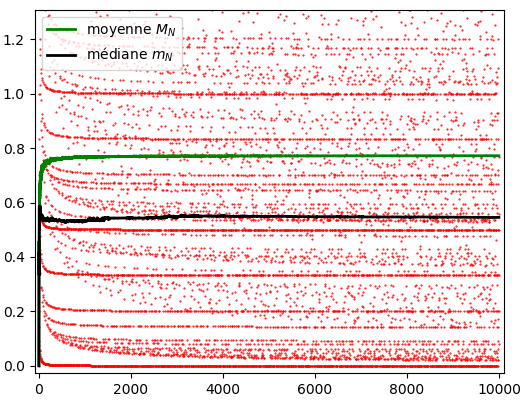
\includegraphics[scale=0.8]{graphedn4.png}
\end{center}
\caption{\footnotesize{ Moyennes et médianes progressives pour $n \le 10000$.}}
\label{nuagen 4}
\end{figure}


% % % % % % % % % % % % % % % % % % % % % % % % % % % % % % % %

\subsection{Autres propriétés}
\begin{prop} \label{prop11}
\begin{equation} \label{eq11} dl^{-1}(1) = \{p^p \mid p \in \Pm \}. \end{equation}
\end{prop}

\Prv \\

\fbox{$\supset$ :}
Conséquence du lemme \ref{lem1}.

\fbox{$\subset$ :}
On raisonnera par l'absurde. Supposons $n \in \N^{*}$ possédant strictement plus d'un diviseur, tel que $dl(n)=1$. On l'écrit sous la forme $n=\prod_{i=1}^{k} {p_{a_i}}^{\alpha_{a_i}}$, avec $k>1$. Alors
\[ \sum_{i=1}^{k} \frac{\alpha_{a_i}}{p_{a_i}} = 1 \]
\[ \sum_{i=2}^{k} \frac{\alpha_{a_i}}{p_{a_i}} = 1 - \frac{\alpha_{a_1}}{p_{a_1}} = \frac{p_{a_1}-\alpha_{a_1}}{p_{a_1}}. \]
Le membre tout à gauche est strictement positif, donc $1 \le \alpha_{a_1} < p_{a_1}$. Le numérateur tout à droite est alors compris dans $[\![1, p_{a_1}-1]\!]$, et sa fraction se retrouve irréductible.\\
Si l'on écrit le membre tout à gauche comme une fraction, son dénominateur $\prod_{i=2}^{k} p_{a_i}$ ne peut pas être réduit en $p_{a_1}$ $\Rightarrow$ contradiction.\\
Puisqu'un antécédent de 1 ne peut avoir qu'un seul facteur premier distinct $p$, il est nécessairement de la forme $n=p^p$. \cqfd \\

\begin{cor} \label{cor4} Sur le graphe de $d$, les seules droites de pente 1 sont celles associées aux $A_{p^p}$ pour p premier. \end{cor}
\Prv Conséquence de (\ref{eq2}). \cqfd \\


\begin{figure}[!ht]
\begin{center}
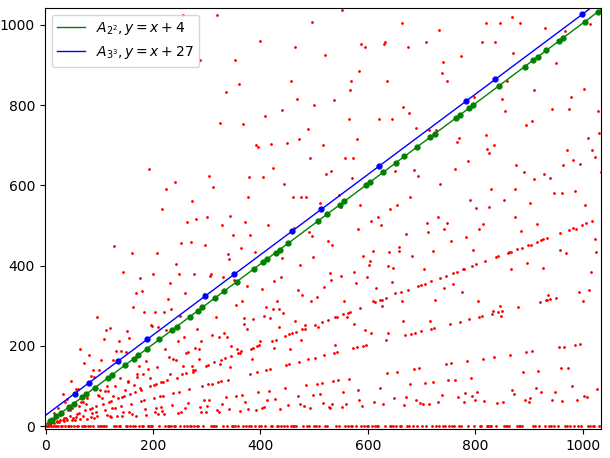
\includegraphics[scale=0.65]{graphed5.png}
\end{center}
\caption{\footnotesize{Illustration du corollaire \ref{cor4} pour $p=2$ et $p=3$.}}
\label{nuage 4}
\end{figure}


Il est intéressant de remarquer que sur les abscisses comprises dans l'intervalle d'entiers $[\![0, N]\!]$, l'ensemble $A_n$ (ou $A'_n$) contient $\pi(\lfloor \frac{N}{n} \rfloor)$ points. Autrement dit,
\[C_n^N = card(A_n \cap ([\![0, N]\!] \times \N)) = \pi(\lfloor \frac{N}{n} \rfloor) \underset{N \to \infty}{\sim} \frac{N}{n\ln(N)}. \]
 Ainsi pour $n$ et $n'$ deux entiers,
\[ \frac{C_n^N}{C_n'^N} \sim \frac{n'}{n}. \]
Sur la représentation, l'ensemble $A_n$ (respectivement $A'_n$) sera donc $\frac{n'}{n}$ fois plus « dense » que l'ensemble $A_{n'}$ (respectivement $A'_{n'}$). \\
Les pentes associées aux entiers les plus petits (cf. table \ref{tab1}) sont les plus visibles sur le graphe de $d$. Sur l'histogramme \ref{nuagen 5} des $N$ premières valeurs de $dl$ et de pas $e$, on aperçoit bien les "raies" auxquelles appartiennent les abscisses des premiers $dl(n)$, avec les hauteurs associées $h_{N,e}(dl(2)) \simeq \frac{\overbrace{h_{N,e}(0)}^{h_{N,e}(dl(1))}} {2}$, $h_{N,e}(dl(3)) \simeq \frac{h_{N,e}(0)}{3}$, $h_{N,e}(dl(4)) \simeq \frac{h_{N,e}(0)}{4} \dots$

\begin{table}[!ht] \label{tab1}
\begin{center}
\begin{tabular}{|c|c|c|c|c|c|c|c|c|c|c|c|c|c|c|c|c|}
\hline
\textbf{n} & \textbf{1} & \textbf{2} & \textbf{3} & \textbf{4} & \textbf{5} & \textbf{6} & \textbf{7} & \textbf{8} & \textbf{9} & \textbf{10} & \textbf{11} & \textbf{12} & \textbf{13} & \textbf{14} & \textbf{15} & \textbf{16}\\
\hline
\textbf{d(n)} & 0 & 1 & 1 & 4 & 1 & 5 & 1 & 12 & 6 & 7 & 1 & 16 & 1 & 9 & 8 & 16 \\
\hline
\textbf{dl(n)} & 0 & $\sfrac{1}{2}$ & $\sfrac{1}{3}$ & 1 & $\sfrac{1}{5}$ & $\sfrac{5}{6}$ & $\sfrac{1}{7}$ & $\sfrac{3}{2}$ & $\sfrac{2}{3}$ & $\sfrac{7}{10}$ & $\sfrac{1}{11}$ & $\sfrac{4}{3}$ & $\sfrac{1}{13}$ & $\sfrac{9}{14}$ & $\sfrac{8}{15}$ & 2\\
\hline
\end{tabular}
\end{center}
\caption{Table des valeurs de $d$ et $dl$ pour $1 \le n \le 16.$}
\label{tab1}
\end{table}

\begin{figure}[ht]
\begin{center}
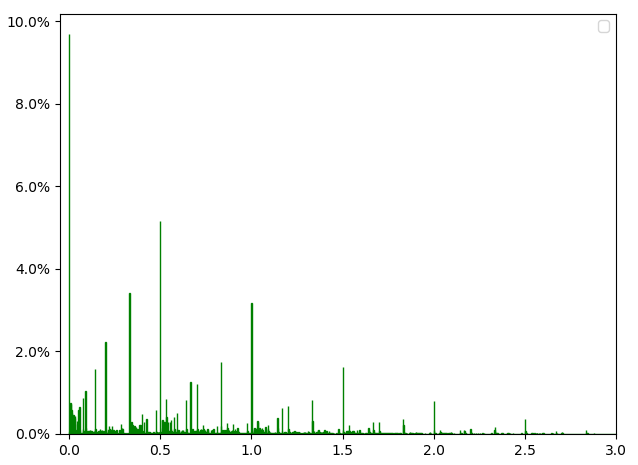
\includegraphics[scale=0.7]{graphedn5.png}
\end{center}
\caption{\footnotesize{Histogramme de présence des $N=30000$ premières valeurs pour un pas $e=0.002$.}}
\label{nuagen 5}
\end{figure}

\begin{conj} $\forall q \in L_d$,
\[ \lim_{\begin{smallmatrix}  e \to 0 \\ N \to \infty \end{smallmatrix}} \frac{h_{N,e}(q)}{h_{N,e}(0)} =  \sum_{a \in dl^{-1}(q)}^{} \frac{1}{a}.\] \end{conj}

% % % % % % % % % % % % % % A FAIRE % % % % % % % % % % % % % % % % %

% bosser sur d(d(n)) et ses points alignés sur la droite de pente y=3/2x + 12 (par ex 2504, 2536, 8312) -> IMAGE, avec la primalité de 3*(leur gd facteur premier)+2 ? Occurence des congruences des nbres premiers mod 3 ? https://oeis.org/A088878




\end{document}